% -*- coding: utf-8 -*-
%\documentclass{article}
\documentclass{ctexart}

\usepackage{CJK}
\usepackage{booktabs}
\usepackage{multirow}
\usepackage{geometry}
\usepackage{upgreek}
\usepackage{amsmath}
\usepackage{indentfirst}
\usepackage{geometry}
\usepackage{upgreek}
\usepackage{fancybox}
\usepackage{indentfirst}
\usepackage{url}
\usepackage{graphicx}
\usepackage{listings}
\usepackage{fancyhdr}
\usepackage{xcolor}
\usepackage{inconsolata}

% COLORS (Tango)
\definecolor{LightButter}{rgb}{0.98,0.91,0.31}
\definecolor{LightOrange}{rgb}{0.98,0.68,0.24}
\definecolor{LightChocolate}{rgb}{0.91,0.72,0.43}
\definecolor{LightChameleon}{rgb}{0.54,0.88,0.20}
\definecolor{LightSkyBlue}{rgb}{0.45,0.62,0.81}
\definecolor{LightPlum}{rgb}{0.68,0.50,0.66}
\definecolor{LightScarletRed}{rgb}{0.93,0.16,0.16}
\definecolor{Butter}{rgb}{0.93,0.86,0.25}
\definecolor{Orange}{rgb}{0.96,0.47,0.00}
\definecolor{Chocolate}{rgb}{0.75,0.49,0.07}
\definecolor{Chameleon}{rgb}{0.45,0.82,0.09}
\definecolor{SkyBlue}{rgb}{0.20,0.39,0.64}
\definecolor{Plum}{rgb}{0.46,0.31,0.48}
\definecolor{ScarletRed}{rgb}{0.80,0.00,0.00}
\definecolor{DarkButter}{rgb}{0.77,0.62,0.00}
\definecolor{DarkOrange}{rgb}{0.80,0.36,0.00}
\definecolor{DarkChocolate}{rgb}{0.56,0.35,0.01}
\definecolor{DarkChameleon}{rgb}{0.30,0.60,0.02}
\definecolor{DarkSkyBlue}{rgb}{0.12,0.29,0.53}
\definecolor{DarkPlum}{rgb}{0.36,0.21,0.40}
\definecolor{DarkScarletRed}{rgb}{0.64,0.00,0.00}
\definecolor{Aluminium1}{rgb}{0.93,0.93,0.92}
\definecolor{Aluminium2}{rgb}{0.82,0.84,0.81}
\definecolor{Aluminium3}{rgb}{0.73,0.74,0.71}
\definecolor{Aluminium4}{rgb}{0.53,0.54,0.52}
\definecolor{Aluminium5}{rgb}{0.33,0.34,0.32}
\definecolor{Aluminium6}{rgb}{0.18,0.20,0.21}

\author{Your Name}
\title{Test Document $L^AT_EX$}

%\pagenumbering{roman}
\pagenumbering{Roman} %显示罗马数字页数
\begin{document}
\begin{CJK*}{GBK}{song}


\maketitle

\section{sec1}
This is a test document
\subsection{sec2}
This is a test document2
\subsubsection{sec3}
This is a test document3
\paragraph{paragraph}
xxxx


\begin{Sbox}
\begin{minipage}{\textwidth}
\begin{verbatim}
the --replicate-* options, can be set only when the slave server starts.
\end{verbatim}
\end{minipage}
\end{Sbox}
\fbox{\TheSbox}

\parbox{17em}{There are two ways to incorporate images into your LaTeX document, and both use the graphicx package by means of putting the command \textbackslash usepackage\{graphicx\} near the top of the LaTeX file, just after the documentclass command.}

\begin{itemize}
\item First thing
\item Second thing
\item Third thing
\end{itemize}

\begin{enumerate}
\item First numbered thing
\item Second numbered thing
\item Third numbered thing
\end{enumerate}

\begin{quote}
There are two ways to incorporate images into your LaTeX document, and both use the graphicx package by means of putting the command \textbackslash usepackage\{graphicx\} near the top of the LaTeX file, just after the documentclass command.
\end{quote}

\begin{description}
\item[First item] text
\item[Second item] dfe df
\item[Third item] dfexxdf
\item[4th item] sxe
\end{description}

\makebox[\textwidth]{\hrulefill}
\begin{verbatim}
#include <iostream>
using namespace std;
int main()
{
    cout<<"hello world"<<endl;
}
\end{verbatim}
\makebox[\textwidth]{\hrulefill}
\begin{verbatim}
from GChartWrapper import Pie
from GChartWrapper import Pie3D

p=Pie3D( [1,2,3,4] ).label('A','B','C','D').color('00dd00')
p.save('a.png')

p=Pie([5,10,15]).title('Hello Pie').color('red','lime').label('hello', 'world','Hello World')
p.save('b.png')
\end{verbatim}
\makebox[\textwidth]{\hrulefill}

\begin{tabular}{|c|c|c|}\hline 
\toprule
aaaaaaa                                             & xetn &ewrsssssss\\ \hline
\multicolumn{2}{|l|}{\multirow{3}*{combined cell}}  &  xdeeee\\ \cline{3-3}
\multicolumn{2}{|l|}{}                              & xeefese\\ \cline{3-3}
\multicolumn{2}{|l|}{}                              & fdsfsdf\\ \hline
fasdfdsf &fdsafasf &fsfsf\\ \hline
\bottomrule
\end{tabular}

\begin{tabular}{|c|c|c|c|}\hline \toprule
\multicolumn{2}{|c|}{aa} & b & b\\ \hline
c&c & b & b \\ \hline
a & a & b & b\\  \hline
\bottomrule
\end{tabular}

\begin{table}[hbtp]
\caption{This table is an example}
\begin{center}
\begin{tabular}{c|c|c}
First row, first column & First row second column & First row, third column \\ \hline
Second row, first column & Second row, second column & Second row, third column \\
Third row, first column & Third row, second column & Third row, third column \\
\multicolumn{3}{c}{78}
\end{tabular}
\end{center}
\label{exampletable}
\end{table}



\begin{figure}[hbtp]
\caption{Img B}
\begin{center}
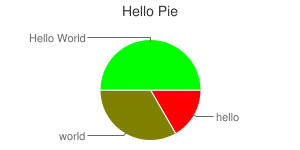
\includegraphics[scale=0.75]{pic/b.png}
\end{center}
\label{fig1}
\end{figure}

\begin{tabular}{l*{6}{c}r}
Team              & P & W & D & L & F  & A & Pts \\
\hline
Manchester United & 6 & 4 & 0 & 2 & 10 & 5 & 12  \\
Celtic            & 6 & 3 & 0 & 3 &  8 & 9 &  9  \\
Benfica           & 6 & 2 & 1 & 3 &  7 & 8 &  7  \\
FC Copenhagen     & 6 & 2 & 1 & 2 &  5 & 8 &  7  \\
\end{tabular}

${\surd}$
${\texttimes}$
\begin{tabular}{| p{5cm} | c |}
        \hline
        \begin{verbatim}
        code
        \end{verbatim}
        & description
        \\ \hline
\end{tabular}
\\
\\
\\
\definecolor{codecolor}{rgb}{0.80,0.91,0.81}
\textcolor[rgb]{0.69,0.94,0.71}{textcolor text}

%\renewcommand{\ttdefault}{DejaVuSansMono}
\renewcommand{\ttdefault}{pcr}
\lstset{
basicstyle=\ttfamily,
language=Python,
breaklines=true,                % sets automatic line breaking
breakatwhitespace=false,        % sets if automatic breaks should only happen at whitespace
title=\lstname,                 % show the filename of files included with \lstinputlisting;
tabsize=4,	
showspaces=false,
showtabs=false,
showstringspaces=false,
showstringspaces=false,
backgroundcolor=\color[rgb]{0.61,0.92,0.69}
}

\begin{lstlisting}[frame=single,
                    framerule=1pt,
                    numbers=left,
                    firstnumber=0,
                    caption={Sample python source code},]
from GChartWrapper import Pie
from GChartWrapper import Pie3D
p=Pie3D([1,2,3,4]).label('A','B','C','D').color('00dd00')
p.save('a.png')
p=Pie([5,10,15]).title('Hello Pie').color('red','lime').label('hello', 'world', "Hello World")
p.save('b.png')
\end{lstlisting}

\lstset{
basicstyle=\ttfamily,
language=C++,
tabsize=4,	
breaklines=true,                % sets automatic line breaking
breakatwhitespace=false,        % sets if automatic breaks should only happen at whitespace
title=\lstname,                 % show the filename of files included with \lstinputlisting;
showspaces=false,
showtabs=false,
showstringspaces=false,
showstringspaces=false,
keywordstyle=\bf\color{blue},
identifierstyle=\bf,
numbers=left,
%背景框
framexleftmargin=10mm,
numberstyle=\color[RGB]{0,192,192},
commentstyle=\it\color[RGB]{0,96,96},
stringstyle=\rmfamily\slshape\color[RGB]{128,0,0},
backgroundcolor=\color[RGB]{245,245,244},
}

\begin{lstlisting}[frame=single,
                    framerule=1pt,
                    numbers=left,
                    language={C++},
                    firstnumber=0,caption={Sample c++ source code}]
const int maxn = 500;
int map[maxn][maxn],t[maxn],p[maxn];
bool isVis[maxn];
int isGirl[maxn];

#include <iostream.h>
#include <memory.h>
void readdata(int n){
	int i,j,s;
	char c;
	for (i = 0;i < n; i++)
	{
		cin >> s;
		while (cin >> c,c != '(');
		cin>>t[s];
		while (cin>>c, c != ')');
		for (j = 0; j < t[s]; j ++)
			cin >>map[s][j];
	}
}
void color(int k)
{
	int i;
	for (i = 0;i < t[k];i ++)
		if (isGirl[map[k][i]] == 0)
		{
			isGirl[map[k][i]] = 3 - isGirl[k];
			color(map[k][i]);
		}

}
bool Find(int k)
{
	int i,j;
	isVis[k] = true;
	for (i = 0;i < t[k];i ++)
		if (p[map[k][i]] < 0)
		{
			p[map[k][i]] = k;
			return true;
		}
		else
			if (!isVis[p[map[k][i]]])
			{
				j = p[map[k][i]];
				p[map[k][i]] = k;
				if (Find(j)) return true;
				p[map[k][i]] = j;
			}
		return false;
}
int main(){
    cout<<"hello world"<<endl;
	int n,i,ans;
	while (cin >> n){
		readdata(n);
		memset(isGirl,0,sizeof(isGirl));
		for (i = 0;i < n;i ++)
			if (isGirl[i] == 0)
			{
				isGirl[i] = 2;
				color(i);
			}
		ans = n;
		memset(p,-1,sizeof(p));
		for (i = 0;i < n;i ++)
		    if (isGirl[i] == 1)
			{
				memset(isVis,false,sizeof(isVis));				
				if (Find(i)) ans --;
			}
		cout<<ans<<endl;
	}
	return 0;
}
\end{lstlisting}



\lstset{
basicstyle=\ttfamily,
language=Haskell,
tabsize=4,	
breaklines=true,                % sets automatic line breaking
breakatwhitespace=false,        % sets if automatic breaks should only happen at whitespace
title=\lstname,                 % show the filename of files included with \lstinputlisting;
showspaces=false,
showtabs=false,
showstringspaces=false,
showstringspaces=false,
keywordstyle=\bf\color{blue},
identifierstyle=\bf,
numbers=left,
%背景框
framexleftmargin=10mm,
numberstyle=\color[RGB]{0,192,192},
commentstyle=\it\color[RGB]{0,96,96},
stringstyle=\rmfamily\slshape\color[RGB]{128,0,0},
backgroundcolor=\color[RGB]{245,245,244},
}
\lstinputlisting[language=Haskell,caption={Sample Haskell source code}]{SimpleParser.hs}


\end{CJK*}
\end{document} 